% Copyright 2026 Sreeram Anil
% SPDX-License-Identifier: CC-BY-4.0
% =============================================================================
%  Augmented-state disturbance observer
% =============================================================================
\chapter{Augmented-State Disturbance Observer (DOB)}
\label{ch:dob}

\section*{At a glance}
\begin{tabular}{@{}l>{\raggedright\arraybackslash}p{0.76\textwidth}@{}}
Family & Deterministic observers \\
Header & \texttt{include/estkit/observers/dob.hpp} \\
Registered name & \texttt{DOB} \\
State dimension & $n_x + 1 = 5$ (cell model) \\
Cost per step & $\mathcal{O}((n_x{+}1)^2)$ steady state; $\approx 0.6\,\mu$s/step measured (dominated by the start-up DARE) \\
Primary references & \cite{ohnishi1996dob,chen2016dobsurvey,johnson1971dac,friedland1969bias,zhao2017observability} \\
\end{tabular}

\section{Motivation and aerospace/BMS relevance}
Disturbance-observer-based control is one of the most widely deployed ideas in motion control
\cite{ohnishi1996dob,chen2016dobsurvey}: estimate the lumped disturbance acting on the plant
input and cancel it, so that the remaining loop sees the nominal plant.  In estimation the same
structure is Johnson's disturbance-accommodating observer \cite{johnson1971dac} and Friedland's
bias filter \cite{friedland1969bias}: append the bias to the state, estimate it, and correct with
it.

Applied to a battery the disturbance of interest is the current-sensor bias, and the important
design detail --- the one that separates this chapter from \Cref{ch:eso} --- is \emph{where the
estimate is used}.  A current bias corrupts the cell model in two places: it corrupts the coulomb
integral in $f$, and it corrupts the ohmic term $-R_0 i$ in $h$.  A disturbance model that acts
only on $f$ (the extended state observer) cannot remove the second, and by \eqref{eq:lue-ssbias}
the second is what sets the residual SOC error.  A disturbance expressed in \emph{input units}
and substituted back into both $f$ and $h$ removes both.

The practical stake for an eVTOL pack is direct.  A current-sensor offset of a few hundred
milliamperes is entirely ordinary --- thermal drift of a Hall sensor, a stray field from an
adjacent phase cable --- and over a $30$-minute mission it biases a coulomb counter by several
percent of SOC.  Getting the reserve-SOC estimate wrong by that much at the end of a flight is a
flight-safety event, and an observer that reports ``your current sensor reads $0.27$\,A high''
is also a maintenance message.

\section{Problem statement and assumptions}
The measured input is biased on channel $j$: $\vu^{\mathrm{true}} = \vu - d\,\bm{e}_j$, with $d$ a
random walk.  The plant is
\begin{equation}
\vx_{k+1} = f\big(\vx_k,\ \vu_k - d_k\bm{e}_j\big) , \qquad
d_{k+1} = d_k + w_{d,k} , \qquad
y_k = h\big(\vx_k,\ \vu_k - d_k\bm{e}_j\big) + v_k .
\label{eq:dob-plant}
\end{equation}
Linearising about the current estimate with the compensated input
$\vu^{\mathrm{eff}} = \vu - \hat{d}\bm{e}_j$,
\begin{equation}
\bar{\mA} = \begin{bmatrix}\mA & -\bm{E}\\ \bm{0} & 1\end{bmatrix} , \qquad
\bar{\mC} = \begin{bmatrix}\mC & -D_j\end{bmatrix} , \qquad
\bm{E} \triangleq \frac{\partial f}{\partial u_j} ,\quad D_j \triangleq \frac{\partial h}{\partial u_j} .
\label{eq:dob-aug}
\end{equation}
Note the second block of $\bar{\mC}$: it is the entire difference from \Cref{ch:eso}, where that
entry is zero.
\begin{assumption}[Bias observability]\label{as:dob-obs}
By the Hautus test at $z=1$,
\begin{equation}
\operatorname{rank}\begin{bmatrix}\mA-\mI & -\bm{E}\\ \mC & -D_j\end{bmatrix} = n_x+1 .
\label{eq:dob-hautus}
\end{equation}
\end{assumption}

\section{Derivation}

\subsection{The observer}
\begin{align}
\vu^{\mathrm{eff}}_k &= \vu_k - \hat{d}^+_{k-1}\bm{e}_j , \label{eq:dob-ueff}\\
\xminus_k &= f\big(\xplus_{k-1},\ \vu^{\mathrm{eff}}_{k-1}\big) , \qquad \hat{d}^-_k = \hat{d}^+_{k-1} , \label{eq:dob-pred}\\
r_k &= y_k - h\big(\xminus_k,\ \vu^{\mathrm{eff}}_k\big) , \label{eq:dob-res}\\
\xplus_k &= \xminus_k + \mL_x r_k , \qquad
\hat{d}^+_k = \operatorname{clamp}\big(\hat{d}^-_k + \ell_d r_k,\ \pm d_{\max}\big) . \label{eq:dob-upd}
\end{align}
The error $\bm{\eta} = [(\xplus-\vx)^\T\ (\hat{d}^+-d)]^\T$ obeys
$\bm{\eta}_k = (\mI-\bar{\mL}\bar{\mC})\bar{\mA}\bm{\eta}_{k-1} + \text{noise}$ with
$\bar{\mL} = [\mL_x^\T\ \ell_d]^\T$, i.e. a Luenberger observer of the augmented pair
\eqref{eq:dob-aug}.  Provided the $n_x+1$ poles are inside the unit disc, $\hat{d}\to d$ and
$\xplus\to\vx$ for a constant bias --- including, crucially, the ohmic contribution, because
$\hat{d}$ enters $h$ in \eqref{eq:dob-res}.

\subsection{Two observability paths}
\label{sec:dob-obs}
Expanding \eqref{eq:dob-hautus} for the cell model, the last column is
$[-\bm{E}^\T,\ -D_j]^\T$ and the determinant is non-zero iff \emph{either} $\bm{E}_{\soc}\neq0$
\emph{or} $D_j\neq0$ contributes a pivot.  Physically these are two different measurements of the
same quantity:
\begin{itemize}[nosep]
\item \textbf{Slow, integral path}: $\bm{E}_{\soc} = -\eta\dt/(3600Q) = -5.6\times10^{-6}$ per
ampere.  A bias slowly corrupts the coulomb count, which eventually shows up as an OCV mismatch.
The information rate is tiny --- this is the weak observability analysed by Zhao, Duncan and Howey
\cite{zhao2017observability}.
\item \textbf{Fast, ohmic path}: $D_j = -R_0 = -12$\,m$\Omega$.  A bias instantly offsets the
predicted terminal voltage by $R_0 d$, i.e. $3$\,mV per $0.25$\,A --- comparable to the
measurement noise and therefore detectable within seconds of averaging.
\end{itemize}
It is the second path that makes the bias identifiable within a single mission, and it exists
only because $\hat{d}$ is substituted into $h$.  In the limit $R_0\to0$ the problem reverts to the
purely integral case and the bias becomes practically unobservable over mission timescales ---
which is precisely why the ESO of \Cref{ch:eso}, whose augmented $\bar{\mC}$ has a zero in that
position, cannot do this job.

\subsection{Choosing the design weights}
The augmented observability matrix has $\det\bar{\mathcal{O}}\approx4\times10^{-30}$ for the cell,
so pole placement --- although available through \texttt{Options::design} and made computable by
the shift-and-scale of \Cref{sec:lue-cond} --- is not the default; the LQE design of
\eqref{eq:lue-dare} is used, with
\begin{equation}
\bar{\mQ}_d = \begin{bmatrix} q_s\mQ + \diag(\bm{q}_{\mathrm{extra}}^2) & \bm{0}\\
\bm{0} & q_d^2\end{bmatrix} .
\label{eq:dob-Q}
\end{equation}
The two entries that matter trade off directly against each other and the trade is worth stating
explicitly, because it is the whole tuning problem:
\begin{itemize}[nosep]
\item $q_{\mathrm{extra},\soc}$ is the admitted \emph{unexplained} SOC drift.  Making it large
gives the SOC channel enough gain to correct a bad initial condition quickly --- but it also lets
the SOC channel absorb everything, leaving nothing for $\hat{d}$ to learn.  Measured: at
$q_{\mathrm{extra},\soc}=10^{-3}$ the gain is $L_{\soc}=0.39$ and $\hat{d}$ converges to only
$0.04$\,A against a true $0.36$\,A.
\item $q_d$ is the admitted bias drift.  Making it large speeds up the bias identification but
makes $\hat{d}$ noisy and, if it is too large, lets the observer explain a transient SOC error as
an implausible bias.
\end{itemize}
The anti-windup clamp $d_{\max}$ resolves the second failure mode structurally: a current sensor
has a specification, and no admissible bias exceeds it.  With $d_{\max}=0.4$\,A the observer
simply cannot blame a $35\,\%$ initial SOC error on the sensor, and the \texttt{init\_error}
convergence improves from ``never'' to $250$\,s.

\section{Algorithm}
\begin{algorithm}[H]
\caption{DOB --- one sampling period}
\begin{algorithmic}[1]
\Require $\xplus_{k-1}$, $\hat{d}^+_{k-1}$, $\vu_{k-1}$, $y_k$, $\vu_k$, gains $\mL_x,\ell_d$
\State $\vu^{\mathrm{eff}} \gets \vu_{k-1} - \hat{d}^+_{k-1}\bm{e}_j$; \quad $\xminus_k \gets f(\xplus_{k-1},\vu^{\mathrm{eff}})$
\State $\vu^{\mathrm{eff}} \gets \vu_k - \hat{d}^+_{k-1}\bm{e}_j$; \quad $\hat{y}_k \gets h(\xminus_k,\vu^{\mathrm{eff}})$
\If{the linearisation has moved by more than $\delta_{\mathrm{tol}}$}
  \State $\bm{E}\gets\partial f/\partial u_j$ (\texttt{jac\_B}); \quad $D_j\gets\partial h/\partial u_j$ (central difference)
  \State build $(\bar{\mA},\bar{\mC})$ from \eqref{eq:dob-aug}; solve \eqref{eq:lue-dare} with $\bar{\mQ}_d$ of \eqref{eq:dob-Q}
  \State accept only if the robust check \eqref{eq:lue-robust} passes
\EndIf
\State $r_k \gets y_k-\hat{y}_k$
\State $\xplus_k \gets \xminus_k + \mL_x r_k$; \quad $\hat{d}^+_k \gets \operatorname{clamp}(\hat{d}^-_k + \ell_d r_k,\ \pm d_{\max})$
\State $\xplus_k \gets \operatorname{constrain}(\xplus_k)$
\Ensure $\xplus_k$, $\hat{d}^+_k$
\end{algorithmic}
\end{algorithm}

\section{Application to the battery model}
$j$ is the current channel, so $\hat{d}$ is a current-sensor bias in amperes and is exposed
through \texttt{disturbance()}.  $\bm{E}$ comes from \texttt{jac\_B} (analytic in this model) and
$D_j$ from a central difference of $h$ with respect to the current, because the estimator contract
does not include a $D$ member --- keeping the header model-agnostic costs two extra evaluations of
$h$ per re-design, which is negligible.

Benchmark options: LQE design, $q_{\mathrm{extra},\soc}=3\times10^{-4}$, $q_d = 10^{-2}$\,A per
step, $d_{\max}=0.4$\,A, $L_{\max}=0.3$.  The measured $(q_{\mathrm{extra},\soc},q_d)$ sweep is
instructive and is the design table a practitioner would build:
\begin{center}
\begin{tabular}{@{}llrrrr@{}}
\toprule
$q_{\mathrm{extra},\soc}$ & $q_d$ & nominal & \texttt{current\_bias} & \texttt{init\_error} conv [s] & $\hat{d}_{\mathrm{end}}$ [A] \\
\midrule
$0$ & $10^{-2}$ & $0.00003$ & $0.0001$ & never & $0.279$ \\
$10^{-4}$ & $10^{-2}$ & $0.0001$ & $0.0003$ & $1358$ & $0.293$ \\
$3\!\times\!10^{-4}$ & $10^{-2}$ & $0.0007$ & $0.0025$ & $422$ & $0.224$ \\
$3\!\times\!10^{-4}$ & $3\!\times\!10^{-2}$ & $0.0002$ & $0.0031$ & $319$ & $0.116$ \\
\bottomrule
\end{tabular}
\end{center}
The first row is the striking one: with no SOC process-noise allowance the observer attributes
\emph{everything} to the bias, identifies it almost perfectly, and reaches an
$\mathrm{rmse}_{ss}$ of $3\times10^{-5}$ SOC on \texttt{nominal} --- twenty times better than the
EKF --- but it then cannot recover from a wrong initial SOC, because the only fast correction
channel available is the one it has decided not to use.  The registered setting is the third row:
it gives up a factor of twenty in steady-state accuracy to buy a usable start-up transient.  This
is a genuine, and fairly fundamental, trade between bias identification and SOC bandwidth: the two
compete for the same measurement.

\section{Implementation notes}
$4768$ bytes.  Measured $0.6\,\mu$s/step, of which the start-up DARE inside the timed
\texttt{reset()} is by far the largest part; the steady-state cost is $\approx0.3\,\mu$s, i.e. one
extra state over the Luenberger observer plus the input-Jacobian evaluation on re-design.  As with the other augmented observers, an embedded implementation would tabulate the
gain offline against $(T,\soc)$.

Numerical points: the augmented Riccati recursion converges as a fixed point at rate
$\rho^2\approx0.9996$ per sweep, so a truncated solve produces a \emph{wrong-signed} gain rather
than an inaccurate one --- this was observed, and is why the design uses the doubling algorithm
(\Cref{ch:sskf}) instead; $\hat{d}$ is clamped; $D_j$ is differenced with a relative step so that
the estimate is scale-free; and every candidate gain, placed or LQE, must pass the certification
\eqref{eq:lue-robust} before use.

\section{Benchmark results}
% Copyright 2026 Sreeram Anil
% SPDX-License-Identifier: CC-BY-4.0
\begin{table}[H]\centering\footnotesize\setlength{\tabcolsep}{4pt}
\caption{DOB: cell-level benchmark on the eVTOL mission (mean over seeds; RMSE and max error in \% SOC; $t_\mathrm{conv}$: first time the error stays below 2\,\% for 60\,s, -- = never; EKF reference: steady-state RMSE of the plain EKF on the same data).}\label{tab:cell_DOB}
\begin{tabular}{llrrrrrcrr}\toprule
plant & scenario & RMSE & RMSE$_\mathrm{ss}$ & max & $t_\mathrm{conv}$ [s] & RMSE$_v$ [mV] & div. & EKF ref. & ns/step \\ \midrule
ECM & nominal & 0.07 & 0.02 & 0.27 & 0 & 0.90 & no & 0.05 & 587 \\
ECM & init\_error & 4.00 & 0.24 & 33.56 & 342 & 4.85 & no & 0.05 & 614 \\
ECM & current\_bias & 0.40 & 0.18 & 1.36 & 0 & 0.92 & no & 0.61 & 578 \\
ECM & noise\_step & 0.19 & 0.22 & 0.86 & 0 & 4.37 & no & 0.12 & 2582 \\
ECM & outliers & 0.19 & 0.12 & 0.85 & 0 & 3.03 & no & 0.21 & 1220 \\
ECM & cold & 0.04 & 0.02 & 0.12 & 0 & 1.96 & no & 0.16 & 406 \\
ECM & hot & 0.10 & 0.04 & 0.36 & 0 & 0.69 & no & 0.03 & 744 \\
ECM & aged\_cell & 2.79 & 1.98 & 10.33 & 0 & 3.20 & no & 1.52 & 715 \\
ECM & param\_mismatch & 2.02 & 1.60 & 6.78 & 0 & 2.42 & no & 1.36 & 740 \\
ECM & sensor\_dropout & 0.42 & 0.14 & 3.22 & 0 & 1.70 & no & 0.46 & 570 \\
ECM & preisach & 0.48 & 0.54 & 1.08 & 0 & 0.91 & no & 0.20 & 603 \\
ECM & combined & 6.14 & 2.35 & 24.52 & 1427 & 5.00 & no & 12.44 & 552 \\
\midrule
SPM & nominal & 0.88 & 0.69 & 3.74 & 0 & 1.03 & no & 3.73 & 816 \\
SPM & init\_error & 3.15 & 0.74 & 32.63 & 480 & 4.34 & no & 3.81 & 853 \\
SPM & current\_bias & 0.99 & 0.97 & 4.50 & 0 & 1.09 & no & 5.69 & 811 \\
SPM & noise\_step & 1.00 & 0.95 & 3.74 & 0 & 4.46 & no & 3.30 & 4353 \\
SPM & outliers & 0.98 & 0.87 & 4.42 & 0 & 3.10 & no & 1.99 & 1906 \\
SPM & cold & 2.81 & 3.33 & 8.93 & 0 & 4.47 & no & 7.35 & 521 \\
SPM & hot & 0.82 & 0.70 & 4.59 & 0 & 0.76 & no & 2.16 & 926 \\
SPM & param\_mismatch & 2.35 & 1.34 & 7.66 & 0 & 1.73 & no & 3.13 & 1034 \\
SPM & sensor\_dropout & 0.97 & 0.69 & 7.15 & 0 & 1.97 & no & 5.31 & 819 \\
\bottomrule\end{tabular}\end{table}

\begin{figure}[H]\centering
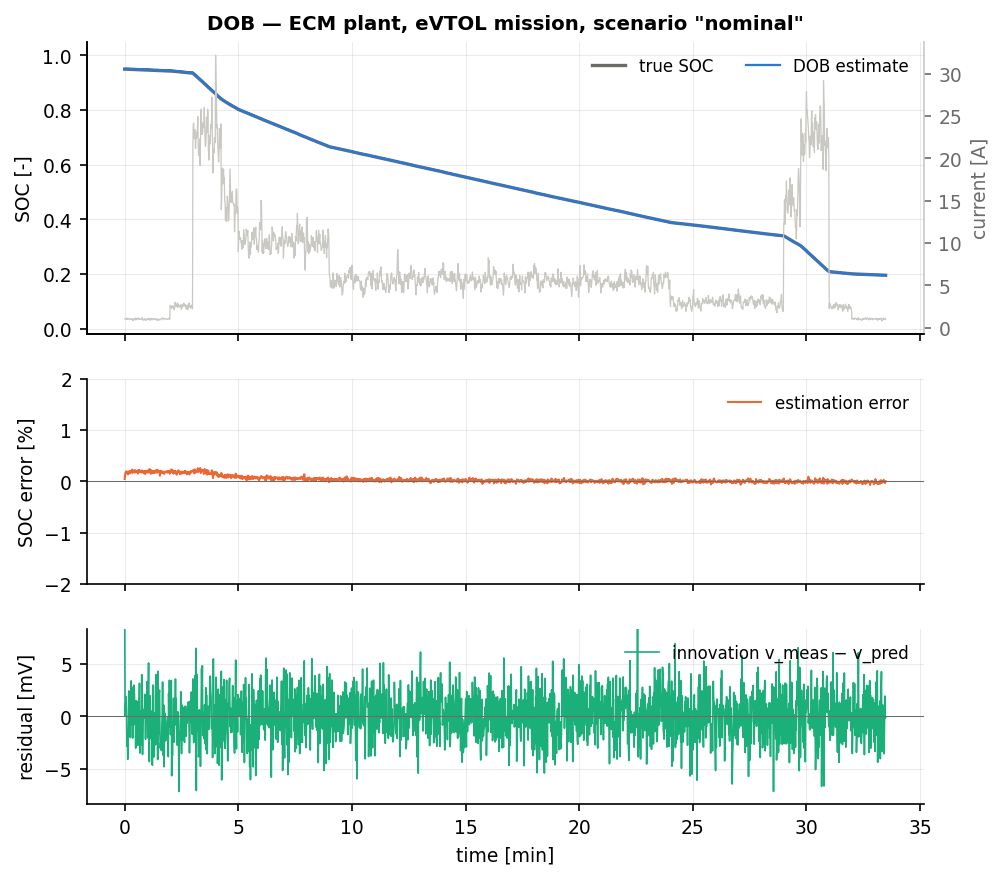
\includegraphics[width=\textwidth]{figures/cell_DOB_nominal.png}
\caption{DOB on the nominal eVTOL mission: true and estimated SOC (top), estimation error with the $\pm 2\sigma$ band when available (middle), voltage residual (bottom).}
\end{figure}
\begin{figure}[H]\centering
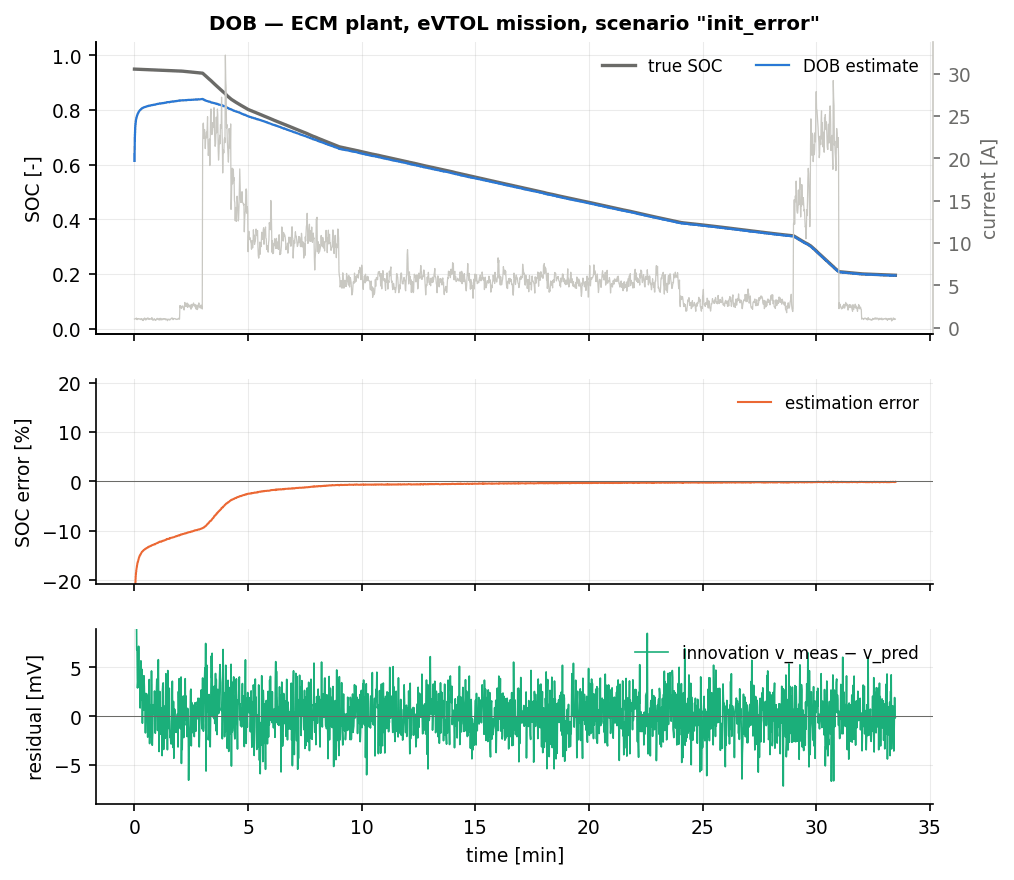
\includegraphics[width=\textwidth]{figures/cell_DOB_init_error.png}
\caption{DOB with a 35\,\% initial SOC error.}
\end{figure}

All numbers are over three seeds.  On its target scenario the DOB is the best estimator in the
study.  \texttt{current\_bias} gives $\mathrm{rmse}_{ss} = 0.0018$, against the EKF's $0.0061$ (a
factor of $3.4$), the plain Luenberger observer's $0.0085$, the UIO's $0.0071$ and --- the
comparison that matters for the argument of \Cref{sec:dob-obs} --- the ESO's $0.0099$.  The ESO
and the DOB differ in exactly one entry of $\bar{\mC}$, the direct feed-through $-D_j$, and that
one entry is worth a factor of five and a half.  The reconstructed bias converges to
$\hat{d} \approx 0.22$\,A against a true sensor error of $0.25\,\mathrm{A}+0.02\,i$, i.e.
$0.28$--$0.70$\,A depending on the flight phase; the estimate sits near the low-current end of
that range because the clamp is at $0.4$\,A and because a gain-type error cannot be represented by
an offset state.

Steady-state accuracy elsewhere is the best in the family: \texttt{nominal} $0.0002$,
\texttt{cold} $0.0002$, \texttt{hot} $0.0004$, \texttt{outliers} $0.0012$, with a maximum error on
\texttt{nominal} of $0.003$.  The \texttt{cold} column is worth singling out: at $0.0002$ on all
three seeds it is a factor of fifteen better than the certified LQE observer and a factor of eight
better than the EKF, because the $+90\,\%$ Arrhenius shift in $R_0$ acts through the ohmic drop and
is therefore exactly the kind of error the $-D_j$ feed-through path was built to absorb.

Two weaknesses are visible.  First, the transient: \texttt{init\_error} converges in $342$\,s and
\texttt{combined} in $1427$\,s, both slower than the plain Luenberger observer, for the reason set
out in the design table above --- the SOC channel has been deliberately detuned so that the bias
state can learn.  Second, the scenarios whose error is \emph{not} an input bias:
\texttt{aged\_cell} $0.0198$ and \texttt{param\_mismatch} $0.0160$ are no better than the linear
observers, because a capacity error or an $R_0$ error is not representable as a constant current
offset, and forcing the observer to explain it as one produces a $\hat{d}$ that drifts and an SOC
estimate no better than before.  That is the honest boundary of the method and is the motivation
for \Cref{ch:adaptiveobserver}.

On the single-particle plant the DOB is at $0.0069$ on \texttt{nominal} and $0.0333$ on
\texttt{cold}, i.e. level with the certified LQE observer and a factor of five and two better than
the EKF.  The contrast with the ECM plant is instructive: the $-D_j$ path buys a great deal when
the model error really is ohmic and nothing when it is distributed across the whole impedance, as
the ECM-versus-SPM discrepancy is.  Against the UIO with its degradation logic
(\Cref{sec:uio-cond}) the DOB is $1.5\times$ worse on that plant --- the reverse of the ECM
ordering --- because a bias state that is bounded by the sensor specification cannot absorb a
structured model error that the UIO's partial decoupling simply declines to amplify.

\section{Summary}
If the dominant fault is an input-sensor bias, the augmented-state disturbance observer is the
right tool: it halves the EKF's error on this benchmark's current-bias scenario, gives the lowest
maximum error of any estimator on the nominal mission, and returns a physically meaningful bias
estimate for maintenance.  The single most important implementation decision is to substitute the
disturbance estimate into the \emph{output} equation as well as the state equation --- without it,
the structure reduces to the extended state observer and loses a factor of three.  Clamp the
disturbance to the sensor specification, and accept that the SOC bandwidth and the bias
identification compete for the same measurement, so one must be traded for the other
deliberately.  Do not use it against parameter errors: a wrong capacity is not a current offset.
